\documentclass[letterpaper]{article}
% Used to do math and such (I think...)
\usepackage{amsmath}
\usepackage{amssymb}

% Used to color text (for todos)
\usepackage{xcolor}

% Used to embed pdfs from yEd and other sources
\usepackage{graphicx}

% Used to embed gnuplot output into document
\usepackage{epstopdf}

% Used to have a table span multiple pages.
\usepackage{longtable}

\usepackage{pdflscape}
\usepackage{geometry}

\usepackage{listingsutf8}
\usepackage{array}
\usepackage{multicol}
\usepackage{multirow}

\usepackage{algorithm}
\usepackage{algpseudocode}

\usepackage{float}

\usepackage{xspace}

\usepackage{subfig}
\usepackage{wrapfig}

% Deal with backwards quotes because evidently Latex doesn't know better.
\usepackage [english]{babel}
\usepackage [autostyle, english = american]{csquotes}
\MakeOuterQuote{"}

\usepackage{mathrsfs}

\DeclareMathOperator{\trace}{Tr}
\DeclareMathOperator{\argmax}{argmax}

\newcommand{\Erdos}{Erd\H{o}s\xspace}
\newcommand{\Renyi}{R\'enyi\xspace}
\newcommand{\Prob}[1]{\mathbb{P}\left( #1 \right)}
\newcommand{\Expected}[1]{\mathbb{E}\left( #1 \right)}

\newcommand{\Derivative}[1]{ \frac{d}{d #1} }
\newcommand{\NDerivative}[2]{ \frac{d^{#2}}{d #1^{#2}}}
\newcommand{\PartialDer}[1]{ \frac{\partial}{\partial #1} }
\newcommand{\NPartialDer}[2]{ \frac{\partial^{#2}}{\partial #1^{#2}} }

\newcommand{\NetworksEq}[2]{Eq. (#1) p. #2 of \textit{Networks} }
\newcommand{\NetworksFig}[2]{Fig. (#1) p. #2 of \textit{Networks} }
\newcommand{\NetworksSec}[2]{\S #1 p. #2 of \textit{Networks}}

\newcommand{\Floor}[1]{\left \lfloor #1 \right \rfloor}

\newcommand{\TODO}[1]{\textcolor{red}{#1}}

\newgeometry{margin=1.125in}

\begin{document}

\title{CSCI-5622: When They Buzz}
\author{Alex Gendreau \and Garrett Lewellen \and Tyler Behm \and a.k.a. Team Skynet}
\date{May 7\textsuperscript{th}, 2015}

\maketitle

\section*{Problem}

\paragraph{} Contestants in a quiz bowl may answer a question as it is being read by buzzing in. We wish to predict when this will happen so that an artificial agent will buzz in just before other contestants. We treat this as two separate problems 1) at what point in the question will the user buzz in, and 2) will the user answer correctly. Correctly answered positions will be reported with a positive sign, and incorrectly negatively. We measure (1) by root mean square error (RMSE) and (2) by sign accuracy (ACC).

\section*{Original Approach}

\paragraph{} We originally proposed a user-dependent probabilistic model based on independence assumptions to report the position with the highest probability given question features. Using logistic regression we found the approach slow and inaccurate (RMSE 106). We pivoted in favor of two simpler parallel lines of work: the Expected Value approach and Right-Wrong approach.

\section*{Expected Value Approach}

\begin{figure}[H]
	\begin{center}
		\resizebox{0.8\linewidth}{!}{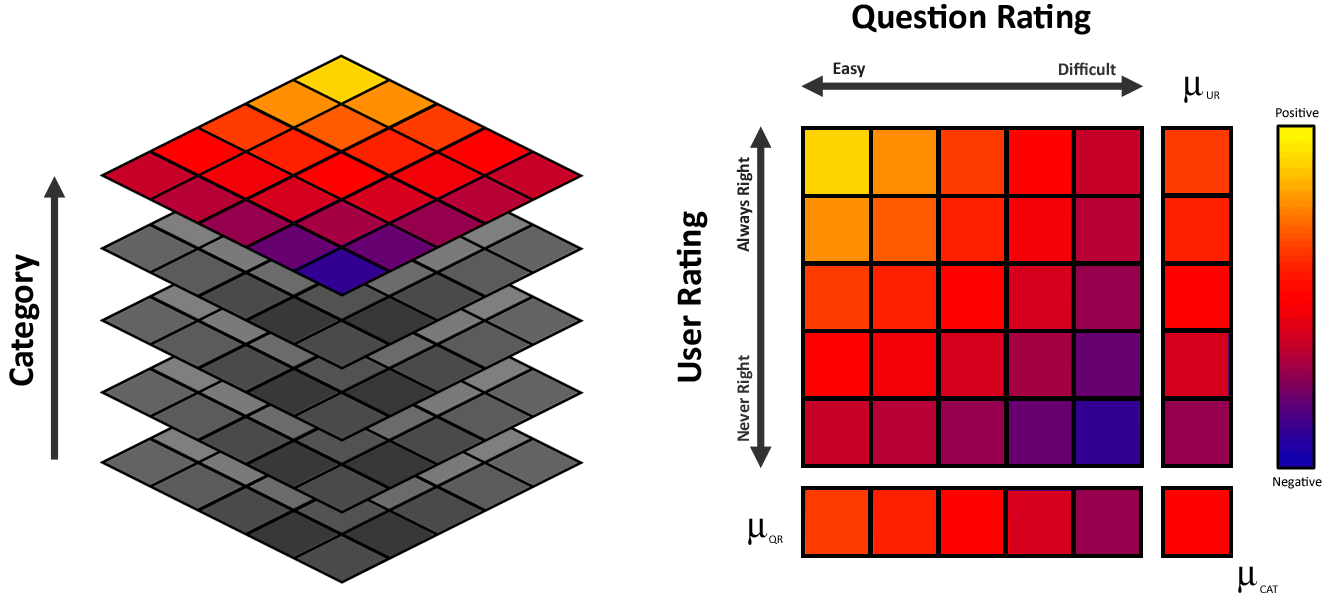
\includegraphics{expectedModel.png}}
	\end{center}
	\caption{Visual representation of the approach. If user rating or question rating are unknown, then expected positions $\mu_{QR}$ and $\mu_{UR}$ are used, or $\mu_{CAT}$ if neither is known.}
	\label{fig:expectedValue}
\end{figure}

\paragraph{} Garrett's simplest approach reported the expected position based on category, user rating, and question rating as depicted in Fig. (\ref{fig:expectedValue}). Users' abilities are measured by the portion of questions they answer correctly denoted by an integer value in $[-7, 7]$. Questions' difficulties are similar, but measured by portion of users who answer them correctly denoted by an integer in $[-2, 2]$. Garrett believed these features ultimately influenced the resulting sign and position. Result: RMSE of 87.48 and ACC of 72.50\%.

\begin{figure}[H]
	\begin{center}
		\resizebox{0.7\linewidth}{!}{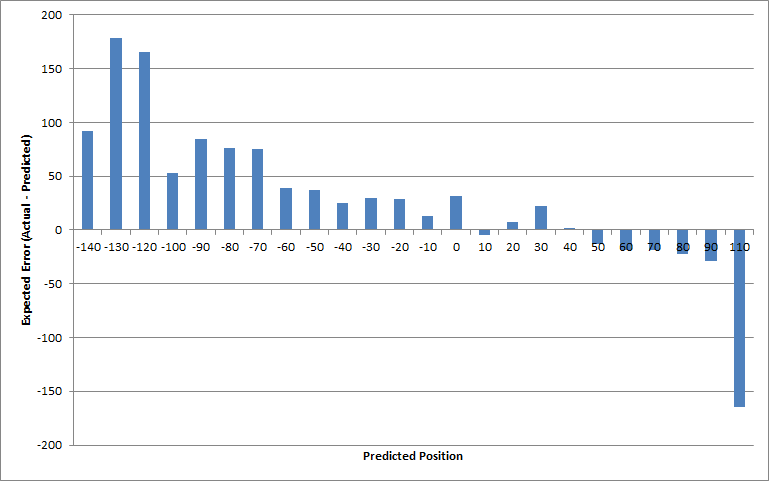
\includegraphics{expectedModelErrorAnalysis.png}}
	\end{center}
	\caption{Expected error as a function of predicted value.}
	\label{fig:expectedValue:errorAnalysis}
\end{figure}

\paragraph{} To improve RMSE, Garrett looked at the relationship between expected error and predicted position. With the intent to zero expected error, he applied these errors as position corrections to produce RMSE of 84.39 and ACC of 73.02\%. Repeating the process three more times yielded RMSE of 83.73 and ACC of 72.65\%. Next, he looked at the most frequently reported position, user rating, and question rating to apply further corrections based on category to obtain RMSE of 83.25 and sign accuracy of 73.5\%.

\begin{figure}[H]
	\begin{center}
		\resizebox{\linewidth}{!}{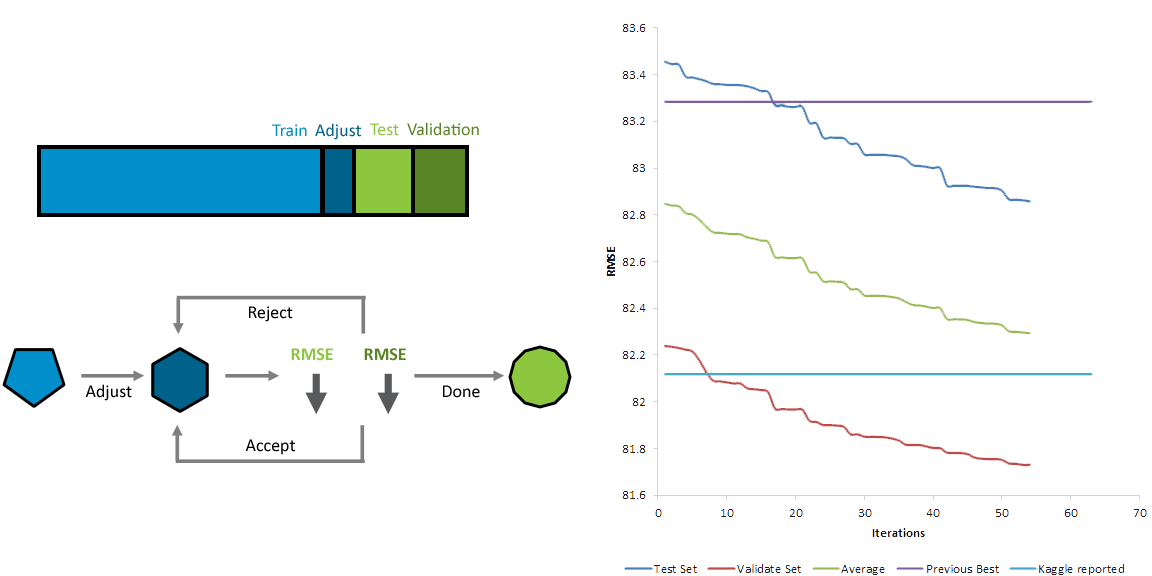
\includegraphics{expectedModelRefinement.png}}
	\end{center}
	\caption{(Left) Visual representation of refinement algorithm. (Right) RMSE as a function of algorithm iteration.}
	\label{fig:expectedValue:refinement}
\end{figure}

Finally, he automated this adjustment process as depicted in Fig. (\ref{fig:expectedValue:refinement}) by splitting the training set into four sets: two to initially fit and adjust the model, and two to verify adjustments reduced RMSE on two separate sets to mimic the Kaggle setup. From the initial fit, examples from the adjustment set are used to make corrections to the model. If RMSE does not improve for both test sets, an adjustment is rejected, otherwise it is accepted, and the process continues until the adjustment set is exhausted. Result: RMSE of 82.11832 as our best Kaggle score until May 2\textsuperscript{nd}.

\section*{Right-Wrong Approach}

\paragraph{} Tyler was the first to realize that incorrectly predicting whether an answer was right or wrong has a higher penalty to the RMSE than the absolute value of the position. This is because of the bimodal distribution of answer positions. See Fig. \ref{fig:categoryPositions}.

\begin{figure}[H]
	\begin{center}
		\resizebox{0.7\linewidth}{!}{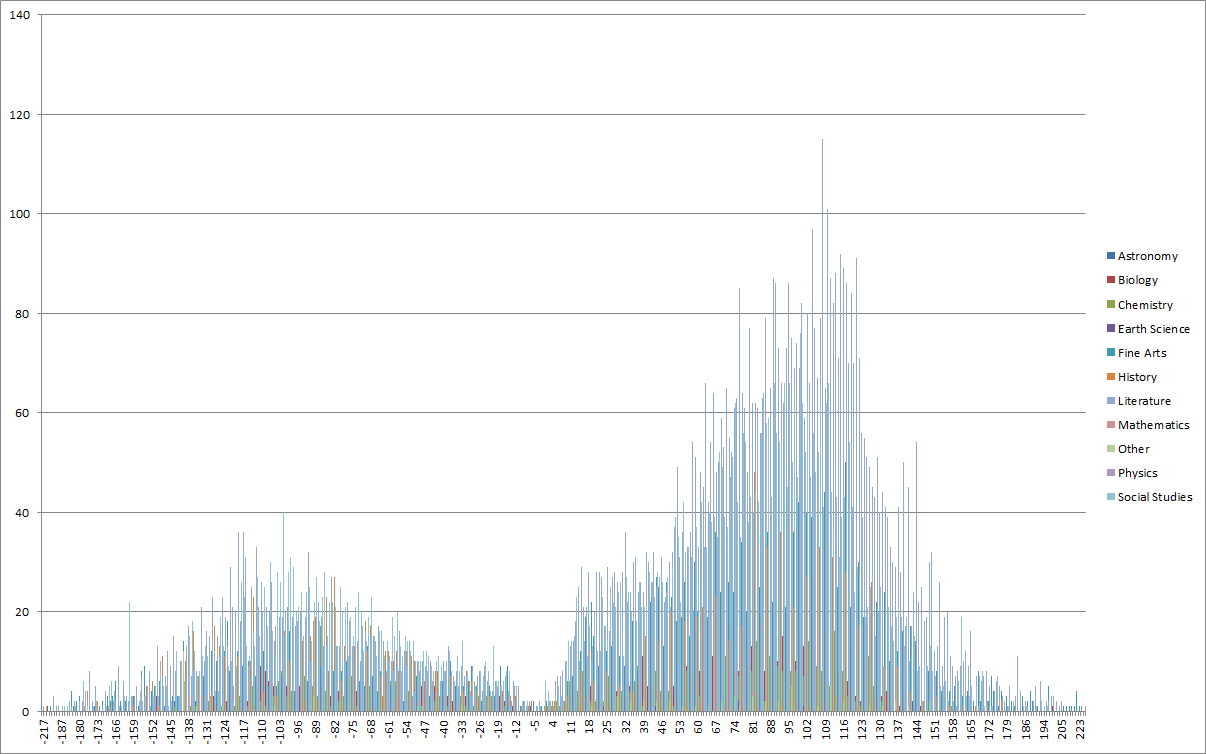
\includegraphics{categoryPositions.png}}
	\end{center}
	\caption{Histogram of frequency of answers binned by answer positions and separated by category.}
	\label{fig:categoryPositions}
\end{figure}

Thus right-wrong predictions warrant their own logistic regression classifier. The following plots motivate the effectiveness of the features. User id was not an effective feature. The histogram shows that most user ids answered few questions. See Fig. \ref{fig:userHisto}. Category was an effective feature. The bar graph shows that the literature category has an average position of twice that of mathematics. See Fig. \ref{fig:categoryAverages}. This could be because literature questions were answered later than math questions, because literature questions were answered correctly more often than math questions, or because of some combination of the two factors. 

Later implementations of the right-wrong approach took the position prediction from the expected value approach as a feature. We tried using it vice-versa (right-wrong as feature into expected) but this was unsuccessful.



\begin{figure}[H]
	\begin{center}
		\resizebox{0.7\linewidth}{!}{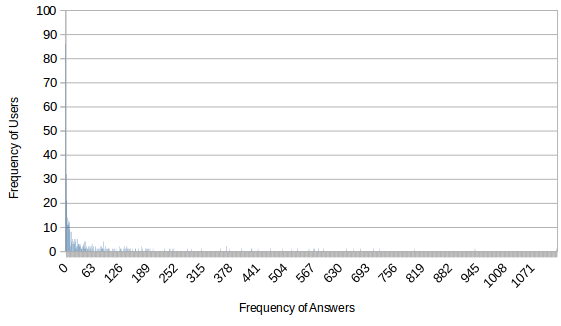
\includegraphics{histogram.png}}
	\end{center}
	\caption{Histogram of frequency of users binned by number of questions they answered.}
	\label{fig:userHisto}
\end{figure}

\begin{figure}[H]
	\begin{center}
		\resizebox{0.7\linewidth}{!}{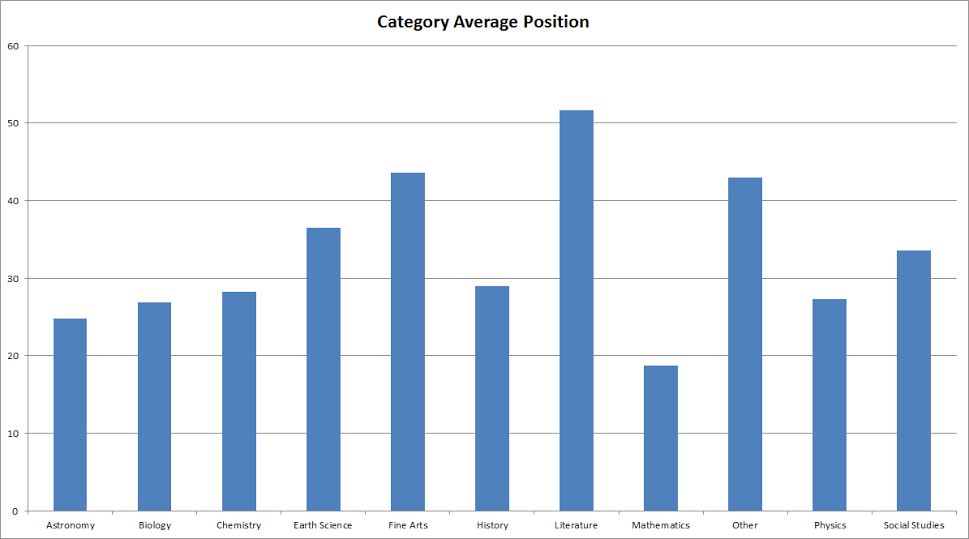
\includegraphics{categoryAverages.png}}
	\end{center}
	\caption{Bar graph of average answer position for each category.}
	\label{fig:categoryAverages}
\end{figure}

The initial implementation of the right-wrong approach modified the original guess file. The original guess file predicted the mean of the training set (39.298062750052644) for all test values. By negating the sign for each prediction in this file, this first implementation by Tyler improved the team's public kaggle score to 84.27541 which was best so far for the team by April 14t\textsuperscript{th}.

Alex helped with the analyser, and Garrett helped with the excel plots that motivated this approach.

Tyler TODO (error analysis)

\section*{Final Approach}

\paragraph{} Because incorrectly predicting whether an answer was right or wrong has such a high penalty, we chose to explore a continuum of correctness predictions. This would allow us to hedge our bets based on how confident was the right-wrong classifier.

\begin{verbatim}
def hedge_bets(guess, conf, mean = 39.298062750052644):
    ## diff is between 0 (no confidence) and 1 (high confidence)
    ## it is the difference in probabilities for predicting yes and no, respectively
    ## output is confidence-weight position guess
    ## the less confident the guess, the more it is dragged towards the mean
    diff = abs(conf[0] - conf[1]) 
    return guess*diff + mean*(1 - diff)
\end{verbatim}

Tyler's first approach of this is shown in the code snippet above. It is a confidence-based linear interpolation towards the mean of the training set. If the right-wrong classifier was $100\%$ certain of its prediction, then the exact position classifier's prediction is returned. If the right-wrong classifier was evenly split between the right and wrong prediction, then the mean is returned. This reduces our risk of increasing the RMSE for low confidence right-wrong predictions.

Alex successfully implemented a better version of this by using lasso regression.

Alex's final model scored the highest for our team and was our final submission.

Alex TODO (Hedge bets, continuous yes/no sign prediction, features, error analysis)

\section*{Conclusions}

\paragraph{} On the public leaderboard, our team placed 4th among 10 teams with a score of 81.55. On the private leaderboard, our team placed 5th with a score of 82.98. Our drop in rank from public to private indicates some degree of overtraining on the public test data.

\end{document}
